\chapter{引言}\label{chap:introduction}

\section{研究背景与意义}

% 问题 -> 
% - 数据中心规模不断扩大
% - 提升利用率的重要性
% 解决方式 -> 混部技术
% - LS 和 BE 应用天然具备混部
% - 通过混部的确解决了问题
% 局限 -> QOS
% 本质 -> 混部共享资源的竞争
% - CPU\Cache\Memory\IO\Net
% - AVX
% 研究现状
% - 劣化监测
% - 调度
% 本文

云计算提供了使用计算资源的便捷方式,其所具备弹性、安全等特征能够减轻云用户的管理负担。随着轻量级虚拟化技术的发展,LXD、Docker等容器技术让应用的分发与部署更加方便,加速了应用上云的进程。同时随着容器编排技术的发展,Kubernetes、OpenShift等提供了更便捷、灵活的运维方式,催生出DevOps概念并逐渐推广。企业与普通用户越来越倾向在云平台上部署应用,不断扩张的需求催生了巨大的云计算市场。而满足庞大的市场需求,云厂商不断扩大数据中心规模,据中国信息通信研究院中国算力发展指数白皮书(2023年)显示,2022年国内数据中心机架规模超过650万个标准机架,基础算力规模达到180EFlops,位居全球第二\citep{chinaict2023}。

数据中心的庞大规模带来了巨大的治理挑战。微软Azure在其内部调研中发现,数据中心每减少1\%的资源分配碎片率,每年就能节省近1亿美元\citep{hadary2020protean}。在数据中心规模不断扩张的背景下,高效利用数据中心计算资源、提高整体资源利用率成为云厂商关注的核心问题。

将互补类型的应用部署到相同物理机上,实现数据中心资源利用率的提升是混部技术的主要方式。依据应用对延迟的敏感度,通常将应用划分为延迟敏感性(LC)与尽力交付型(BE)两类。其中,LC应用通常为交互型应用,这类应用对延时十分敏感,且需要保持运行,如在线购物等。BE应用通常为离线应用,这类应用对延迟几乎没有要求,允许中断和重新运行,如大数据处理等。LC应用负载具有明显潮汐特征,向LC应用的各个空闲时段填充BE应用是混部技术提升资源利用率的核心。阿里云在实践中利用混部技术分别将集群的平均CPU利用率和内存资源利用率提升到了38.2\%和88.2\%\citep{guo2019limits}。

\begin{figure}[!htbp]
    \centering
    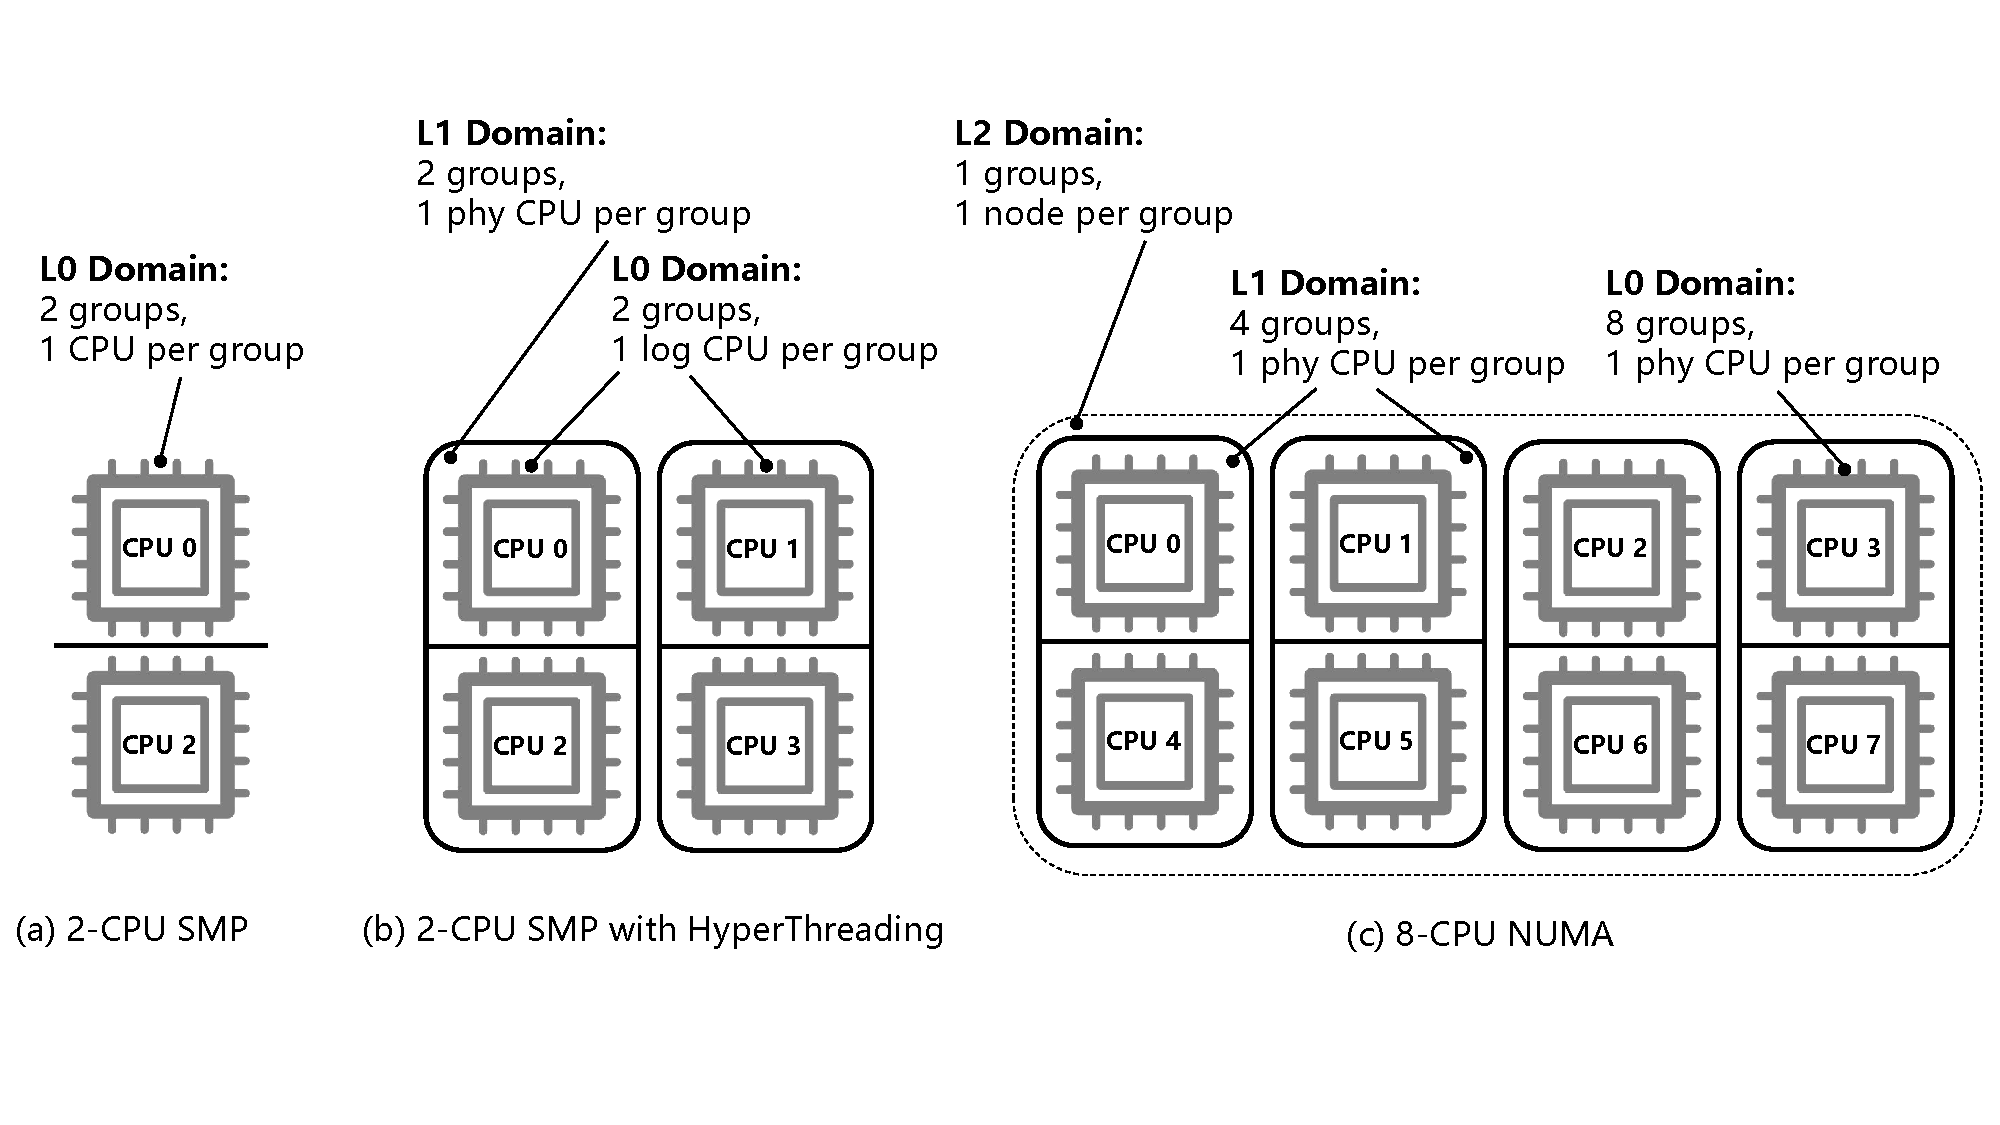
\includegraphics[width=0.85\textwidth]{scheduling_domain}
    \bicaption{\quad CPU拓扑}{\quad CPU Topology}
    \label{fig:scheduling_domain}
\end{figure}

资源竞争是混部技术下不可忽略的问题,分析这一问题首先需要了解资源的共享性与有限性。应用运行在不同的CPU上,CPU拓扑描述了核心之间的物理连接和组织方式,并反映出CPU资源的共享关系。随着CPU设计与制造技术的不断进步,当前出现如超线程技术(Hyper-threading)、非同一内存访问架构(NUMA)、大小核心架构等新特性,CPU拓扑也越来越复杂。常见的CPU拓扑如图~\ref{fig:scheduling_domain}所示,逻辑核位于CPU拓扑的最低一层,任务分时复用逻辑核资源,某一时刻仅有一个任务在运行,彼此几乎没有影响。超线程技术最早于2002年由Intel提出,通过增加部分片上资源使得一个物理核上能够运行多个逻辑核。超线程技术下的片上资源分布如图~\ref{fig:cpu_topology}所示,兄弟核心拥有各自独立的寄存器组与中断控制器,但彼此共享了执行单元、Cache和总线等其他资源。NUMA(非一致存储器访问)架构中存在多个CPU模块,每个CPU模块可包含多个CPU,这些CPU拥有自己的本地内存与IO接口,但彼此共享了相同的内存总线与LLC,且在IO资源上相互竞争。

\begin{figure}[!htbp]
    \centering
    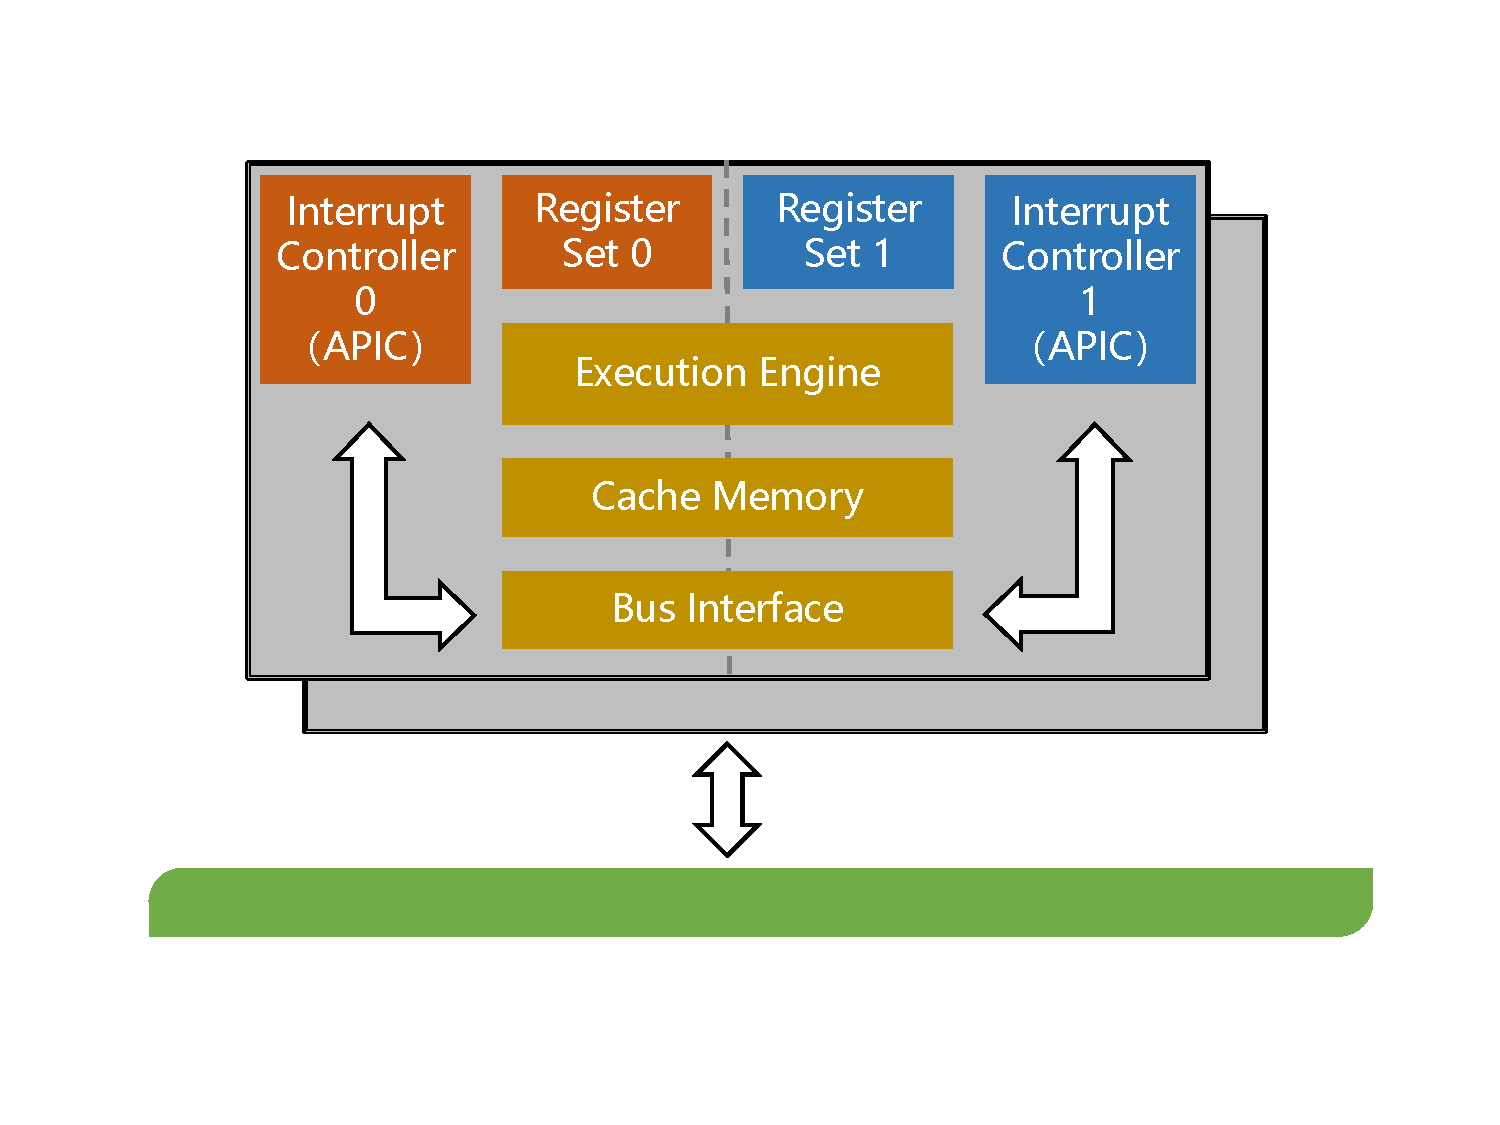
\includegraphics[width=0.5\textwidth]{cpu_topology}
    \bicaption{\quad Siblings片上共享资源 }{\quad Siblings on-chip shared resources}
    \label{fig:cpu_topology}
\end{figure}

现代服务器计算资源丰富,支持大量应用同时运行,然而服务器局部硬件资源有限,如片上资源、LLC、内存带宽、网络带宽等都存在明确的限制。混部技术向单一物理机上部署了更多的任务,增大了局部硬件资源竞争的概率,并容易造成应用QoS的劣化。如在网络子系统中,没有竞争到足够网络带宽的任务会在队列中积压,并导致应用延迟的激增。数据中心应用数量多、软件环境复杂,不同应用对资源的需求各不相同,一方面应用间存在隐含的资源竞争,另一方面应用竞争不同资源所引发的QoS劣化程度也存在差异。

资源竞争引发的QoS劣化体现在应用的性能指标上。云厂商提供了SLO来允许用户定义云应用的期望状态。SLO包含服务可用性、带宽等基础指标,以及每秒请求数量、尾延迟等业务性能指标。云厂商通过与用户协商SLO来提供云产品QoS的保证,并在违反SLO时进行补偿。应用的QoS劣化不仅会为云厂商带来经济损失,还会引发用户的流失,因此保障应用QoS是混部场景下云厂商核心需求。混部场景下QoS保障相关研究通常从三个方向展开:

\begin{enumerate}

    \item 利用可观测性技术来对应用进行劣化监测,同时收集数据以进行画像分析。云厂商依赖可观测性基础设施来对数据中心进行持续监测。可观测性基础设施围绕不同的软件环境设计,如面向虚拟机、面向容器编排系统等。通过全面地指标监测实时收集数据,不仅可以及时发现应用的QoS劣化并进行预警,还能够利用丰富的指标数据来进行细致的画像分析,挖掘更多的混部机会。Google在2011年公布了混部集群监控数据集,阿里云也在2017年公开了一部分混部集群的监控数据集\citep{guo2019limits},这些来自生产环境的脱敏数据集,大大促进了基于数据分析的QoS劣化监测研究。

    \item 围绕资源隔离的混部场景QoS保障研究。资源隔离即通过软硬件手段来强化混部场景下应用在共享资源上的隔离性,防止因敏感资源竞争导致的应用QoS劣化。不同资源隔离技术的区别在隔离资源的类型与粒度上,如使用Cgroup技术对CPU资源隔离,或使用Traffic Control技术\citep{hubert2002linux}对网络带宽隔离。同时,基于硬件级资源隔离技术能实现更细粒度的隔离效果,如隔离末级缓存与内存带宽。组合这些隔离技术来制定不同的调度策略是基于资源隔离混部研究的主要方式。

    \item 围绕任务调度的混部场景QoS保障研究。任务在被调度到CPU上时才能执行,并进一步申请其他的硬件资源,因此CPU资源是大部分硬件资源分配的起点。相关研究从任务调度延时与灵活性上展开。其中微秒级调度机制通过远低于应用延迟要求的调度延时,及时分配CPU资源来避免QoS劣化。灵活的任务调度机制通过修改任务调度的逻辑,针对混部场景应用与硬件特性进行适量身定制,从而更好地进行QoS保障。

\end{enumerate}

% 而了解应用的状态变化,实施精准的调度是解决混部场景中QoS保障问题的核心

\section{国内外相关研究}

\subsection{数据中心可观测性与劣化监测研究现状}

% 可观测性系统
% - 定义
% - 实践

可观测性技术指通过指标监控、日志记录、链路追踪和其他数据收集手段来描述系统的状态,协助理解和诊断系统的行为和性能。在指标监控上,开源社区Prometheus\citep{brazil2018prometheus}定义了一种时序数据结构Metric,以及围绕Metric的高效的编解码机制、灵活的数据存储方式和便捷的PromQL查询语言。此外,Prometheus社区还提供了采集系统的标准实现,包含Promethues Server、Node Exporter等核心组件,并与Grafana社区协作推出开源的数据展示服务。Promethues完全开源且致力于完善多语言库支持。在各云厂商及开源社区开发者的共同参与下,Prometheus社区发展迅速,并逐渐成为指标采集领域的现行标准。

随着软件架构的迭代,可观测性技术也在不断进步。微服务是数据中心常见的软件架构,其中一次请求调用链路往往跨越多个进程与服务器。传统的进程观测手段难以有效地对微服务进行观测,而为解决这一问题,Google在2010年提出了分布式链路追踪系统Dapper\citep{sigelman2010dapper},用于对微服务应用进行性能分析。Dapper的设计如图~\ref{fig:dapper_trace}所示,其中Trace用来记录一次完整的链路追踪,Span用来记录链路中的单个操作。单个操作可以是一次函数的调用或者一段代码块,Dapper需要在代码插桩以指示Span的生成。在函数调用的过程中,Span会作为上下文的一部分传递,并自动地构建调用关系。而微服务中一次函数调用也可以是一次远程过程调用(RPC),此时Dapper会将Span注入到网络报文的载荷中,让Span跨进程、服务器地传递下去。Span最终发送到Dapper的分析系统,并根据树形关系重建得到完整的Trace,实现一次链路追踪过程。OpenTracing和OpenTelemetry等开源项目吸收了Dapper的核心思想,并在云原生社区中迅速推广。链路追踪依赖代码插桩,对编译型语言来说需要修改源代码,因此接入十分不便。而在容器编排系统中则通过Overlay Network来实现无侵入的微服务性能观测。Kubernetes中提供了CNI(Container Network Interface)\citep{k8s-network-plugins},允许开发者自定义容器网络模型。开源CNI项目Cilium\citep{cilium}基于eBPF、Envoy等技术\citep{ebpf,envoyproxy}实现集群的Overlay Network,提供从L3、L4到L7的网络观测能力,并无需侵入用户代码。

\begin{figure}[H]
    \centering
    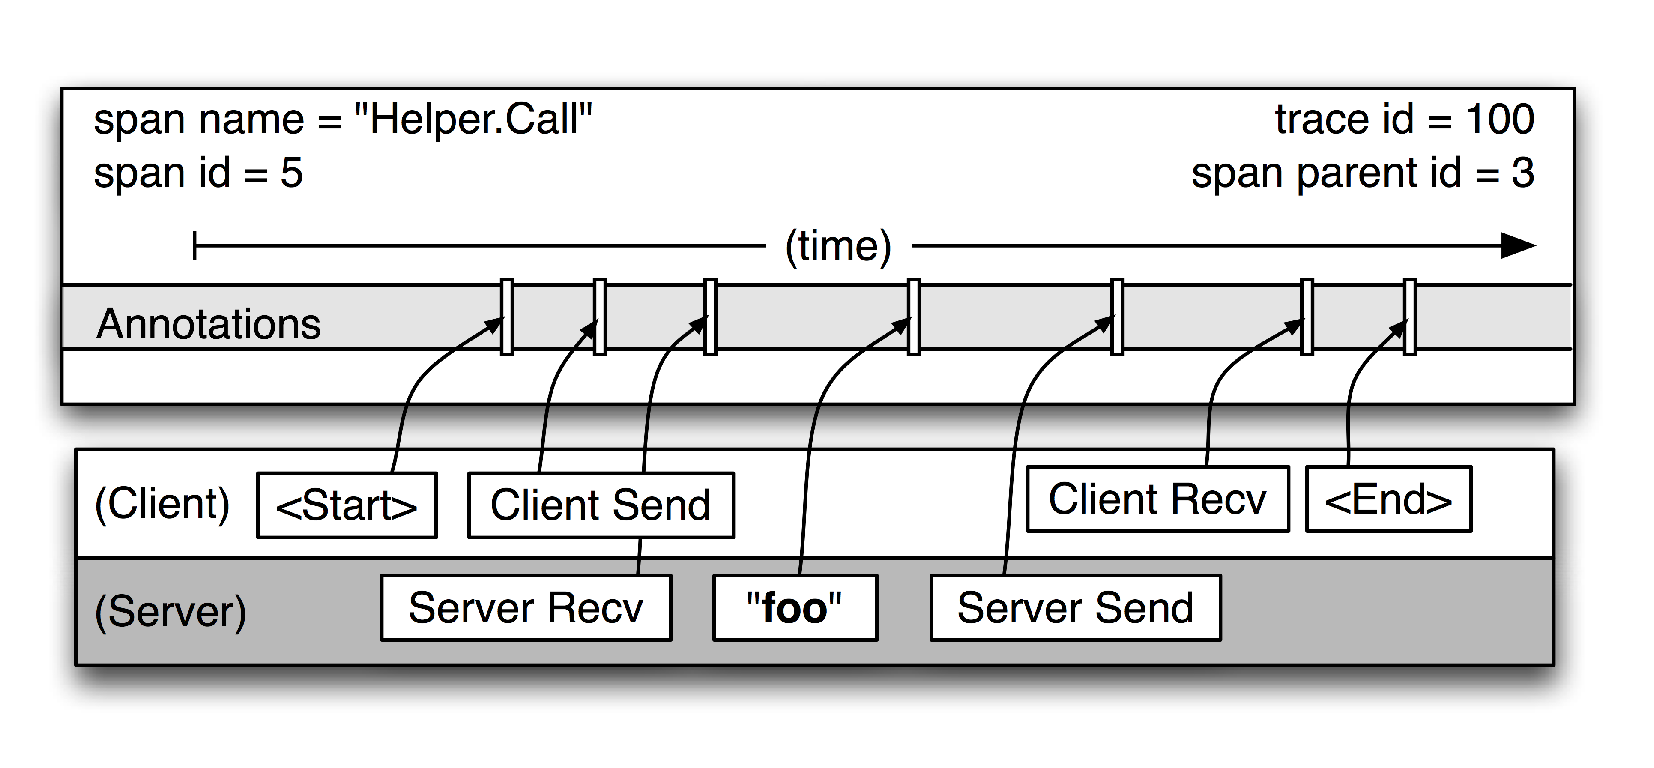
\includegraphics[width=0.6\textwidth]{dapper_span}
    \bicaption{\quad Dapper链路追踪流程(图片引用自文献\citep{sigelman2010dapper})}{\quad Dapper tracking process (picture quoted from paper\citep{sigelman2010dapper})}
    \label{fig:dapper_trace}
\end{figure}

近年来随DevOps技术的发展,可观测性技术在云服务中占据了越来越重要的地位。而基于采集得到的指标分析应用性能劣化情况是可观测系统的主要应用场景。云厂商在早期实践中倾向一些简单的指标。如Google就使用CPI(Cycle Per Instruction)\citep{zhang2013cpi2}来反映应用的性能。CPI本身用于度量微观体系结构下的性能。应用正常运行时CPI通常会在一个小范围内波动。而当应用性能劣化时,CPI波动范围则会显著变化。CPI作为一个简单指标在许多场景都有效,但在CPU频率较低时会出现一定误差。Li Yi等人\citep{yi2020cpi}观察到这一现象,在CPI基础上优化得到RCPI,并修正了误差。

数据中心的监控数据数量多、维度广,支持多样的手段来进行数据分析。近年来随AI技术的发展, 结合AI技术和数据中心QoS劣化监测的研究不断展开。相关研究的核心在于如建立AI模型来预测应用的QoS劣化,从而实现提交发现和预先调度\citep{qiu2020firm, zhou2022aquatope, wang2022deepscaling, gan2021sage, ghafouri2020survey,zheng2020web,wu2019posterior}。其中
FIRM\citep{qiu2020firm}面向Kubernetes集群设计了一种两级的机器学习模型,能精准预测集群中应用的QoS劣化。Di Wu\citep{wu2020data}则提出了一种数据特性感知潜在因素(DCALF)模型来实现高精度的QoS预测,同时能针对不同数据的特点区别地处理。以上研究在调度延时不敏感、应用变化相对慢的集群取得了相当显著的QoS劣化监测与调度效果。

\subsection{围绕资源隔离的混部场景QoS保障研究现状}

% 集群维度: 放置策略
% 单点维度: 细粒度分配

数据中心的资源通常可划分为集群资源与节点资源。其中,集群资源天然通过不同的机器、机架隔离开,相关研究侧重于解决应用的放置问题。集群中各节点都部署了可观测性基础设施,能汇总各节点的资源使用情况。当应用需要调度时,集群调度器通过评估各节点的资源使用情况和应用的资源需求,来选择合适的节点进行部署。集群调度器算法能否给应用分配足够的资源是影响应用QoS的关键。Protean\citep{hadary2020protean}是微软Azure的集群调度器,主要负责用户虚拟机的调度。Protean的决策过程包括地域、地区、机柜三个层次。每一层都设置独立的算法,依据当前层的资源分配情况进行决策,并逐层求解出最优位置。Protean最终选定的位置能够确保为虚拟机提供足够的资源,从而保障虚拟机的QoS。

节点资源有一定的隔离性,同时存在丰富的软硬件手段来进一步强化隔离性。软件上,Linux各资源子系统提供了丰富的资源隔离机制,包括Cgroup、Traffic Control等。硬件上,芯片制造厂商通过在硬件上引入额外特性,实现更细粒度的隔离机制。如针对内存带宽、末级缓存等资源,各大CPU厂商均提供了相关的硬件调控技术,包括Intel Resource Director Technology(Intel RDT)\citep{guide2011intel}、AMD Platform Quality of Service Extensions(AMD PQoS)\citep{amdpqos}、ARM Memory System Resource Partitioning and Monitoring(ARM MPAM)\citep{armmpam}等。节点上更细粒度的资源隔离手段能够有效协助解决"吵闹邻居"问题\citep{xu2018dcat, maricq2018taming, rzadca2020autopilot, kwon2020dc}。

\begin{figure}[!htbp]
    \centering
    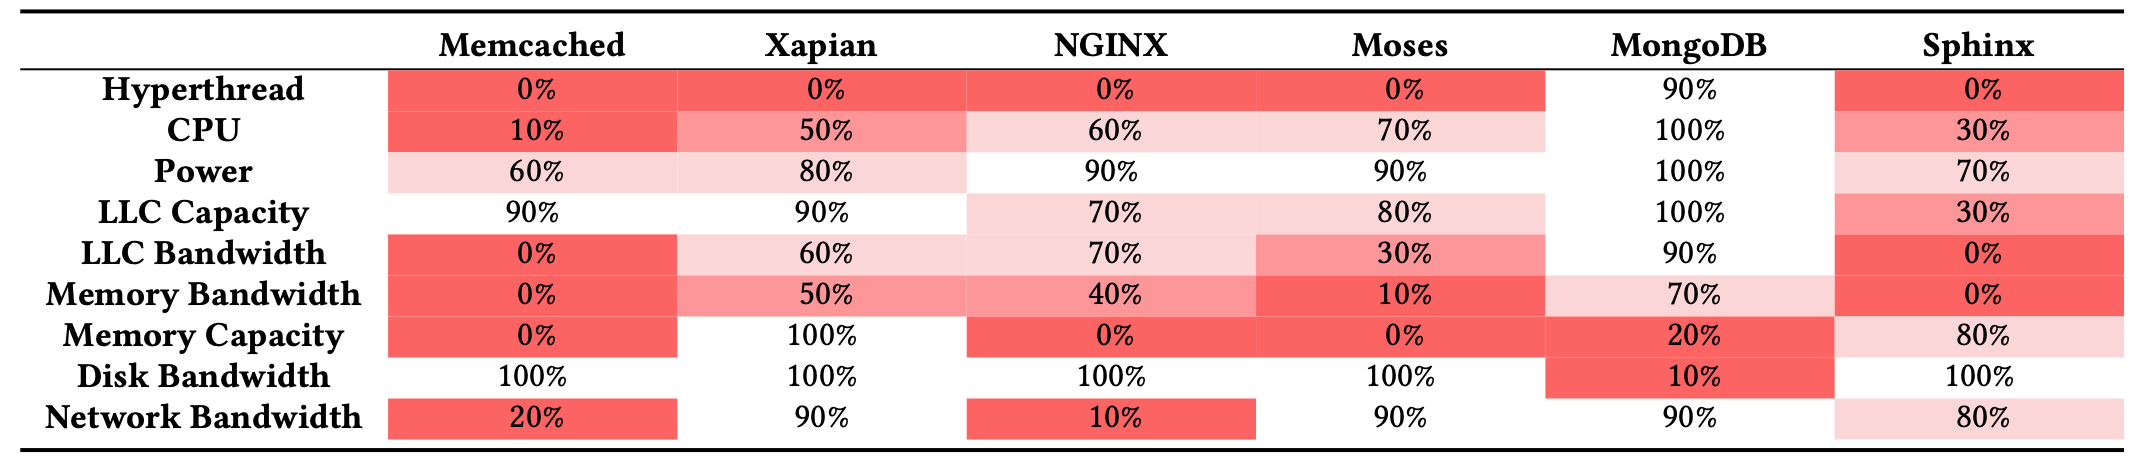
\includegraphics[width=0.85\textwidth]{parties_app_dif}
    \bicaption{\quad 不同资源干扰对应用性能的影响(图片引用自文献\citep{chen2019parties})}{\quad diferent resource interference on application performance(quoted from paper\citep{chen2019parties})}
    \label{fig:parties_app_dif}
\end{figure}

基于节点资源的隔离性,部分研究围绕放置策略展开。Paragon\citep{delimitrou2013paragon}将推荐系统中常用的协同过滤技术(Collaborative filtering technique)引入到放置问题中,通过预测应用对节点上其他应用的影响以及应用能够承受的干扰,来进行应用的放置决策,实现了大多数工作负载场景下的QoS保障。而结合丰富的节点资源隔离手段,部分研究通过避免应用在关键资源上的竞争来实现应用的QoS保障。Quasar\citep{delimitrou2014quasar}预先对应用进行画像分析,并建立分类模型。随后通过分类模型快速确定新应用的资源需求以及干扰的敏感度,并利用资源隔离技术来调整资源分配。Heracles\citep{lo2015heracles}从应用资源敏感度的角度入手,分析了不同应用在不同负载下对于多种资源的敏感度,并依据分析结果优先保证敏感资源供给,从而实现应用的QoS保障。Parties\citep{chen2019parties}则进一步分析了如图~\ref{fig:parties_app_dif}所示更丰富的资源种类。在调度上,不同于Heracles,Parties利用应用间的资源拆借,实现保障应用QoS的同时整体资源利用率也得到提升。CLITE\citep{patel2020clite}利用贝叶斯优化构建资源隔离模型,将多个LC应用与BE应用进行混部,并利用Intel MBA技术对内存带宽进行控制以保障LC应用的QoS。LIBRA\citep{zhang2021libra}则基于一种新型硬件节流机制,实现内存带宽的动态调控,并根据应用的需求变化动态调整,及时地保障内存带宽资源供给。

\subsection{围绕任务调度的混部场景QoS保障研究}

% 内核任务调度
% 微秒级调度

围绕任务调度的QoS保障研究聚焦于CPU资源的分配,相关研究围绕调度机制的设计展开。调度机制的核心在于调度延时与调度策略,其中调度延时通常与Runtime的实现相关,而调度策略则取决于不同混部场景的调度目标。

CFS调度器\citep{pabla2009completely}于2009年提出,用来解决交互式应用与非交互式应用在调度上的公平性问题。CFS的核心在于CPU vruntime的计算与维护。CFS调度器为Run Queue中的每一个调度实体维护一个时间记账,并在每个时钟中断处理中更新。而在每个调度循环中,CFS会调度Run Queue中vruntime最小的任务执行。CFS调度器长期以来都是Linux的默认调度器,但存在灵活性的不足,难以满足当前数据中心应用的需求。为解决CFS的灵活性问题,Linux 6.6版本中引入了EEVDF(Earliest Eligible Virtual Deadline First)调度器。EEVDF调度器\citep{stoica1995earliest}于1995年提出,其中调度器会为每个进程维护一个虚拟截止时间,并在每次调度时选择最早截止时间的任务执行。不同于CFS,EEVDF调度器的优先级设计考虑到了应用对时间片的不同需求,并增加了latency-nice机制。如图~\ref{fig:eevdf_scheduling}所示,为任务设置较高的latency-nice值会让任务总是获得长而少的时间片,这样能够减少上下文切换的次数,对于计算密集型的应用而言有利于提高吞吐。而为任务设置较低latency-nice值则会让任务总是获得短而多的时间片,这样能够让CPU资源更快地分配,从而提升应用的响应度。

\begin{figure}[!htbp]
    \centering
    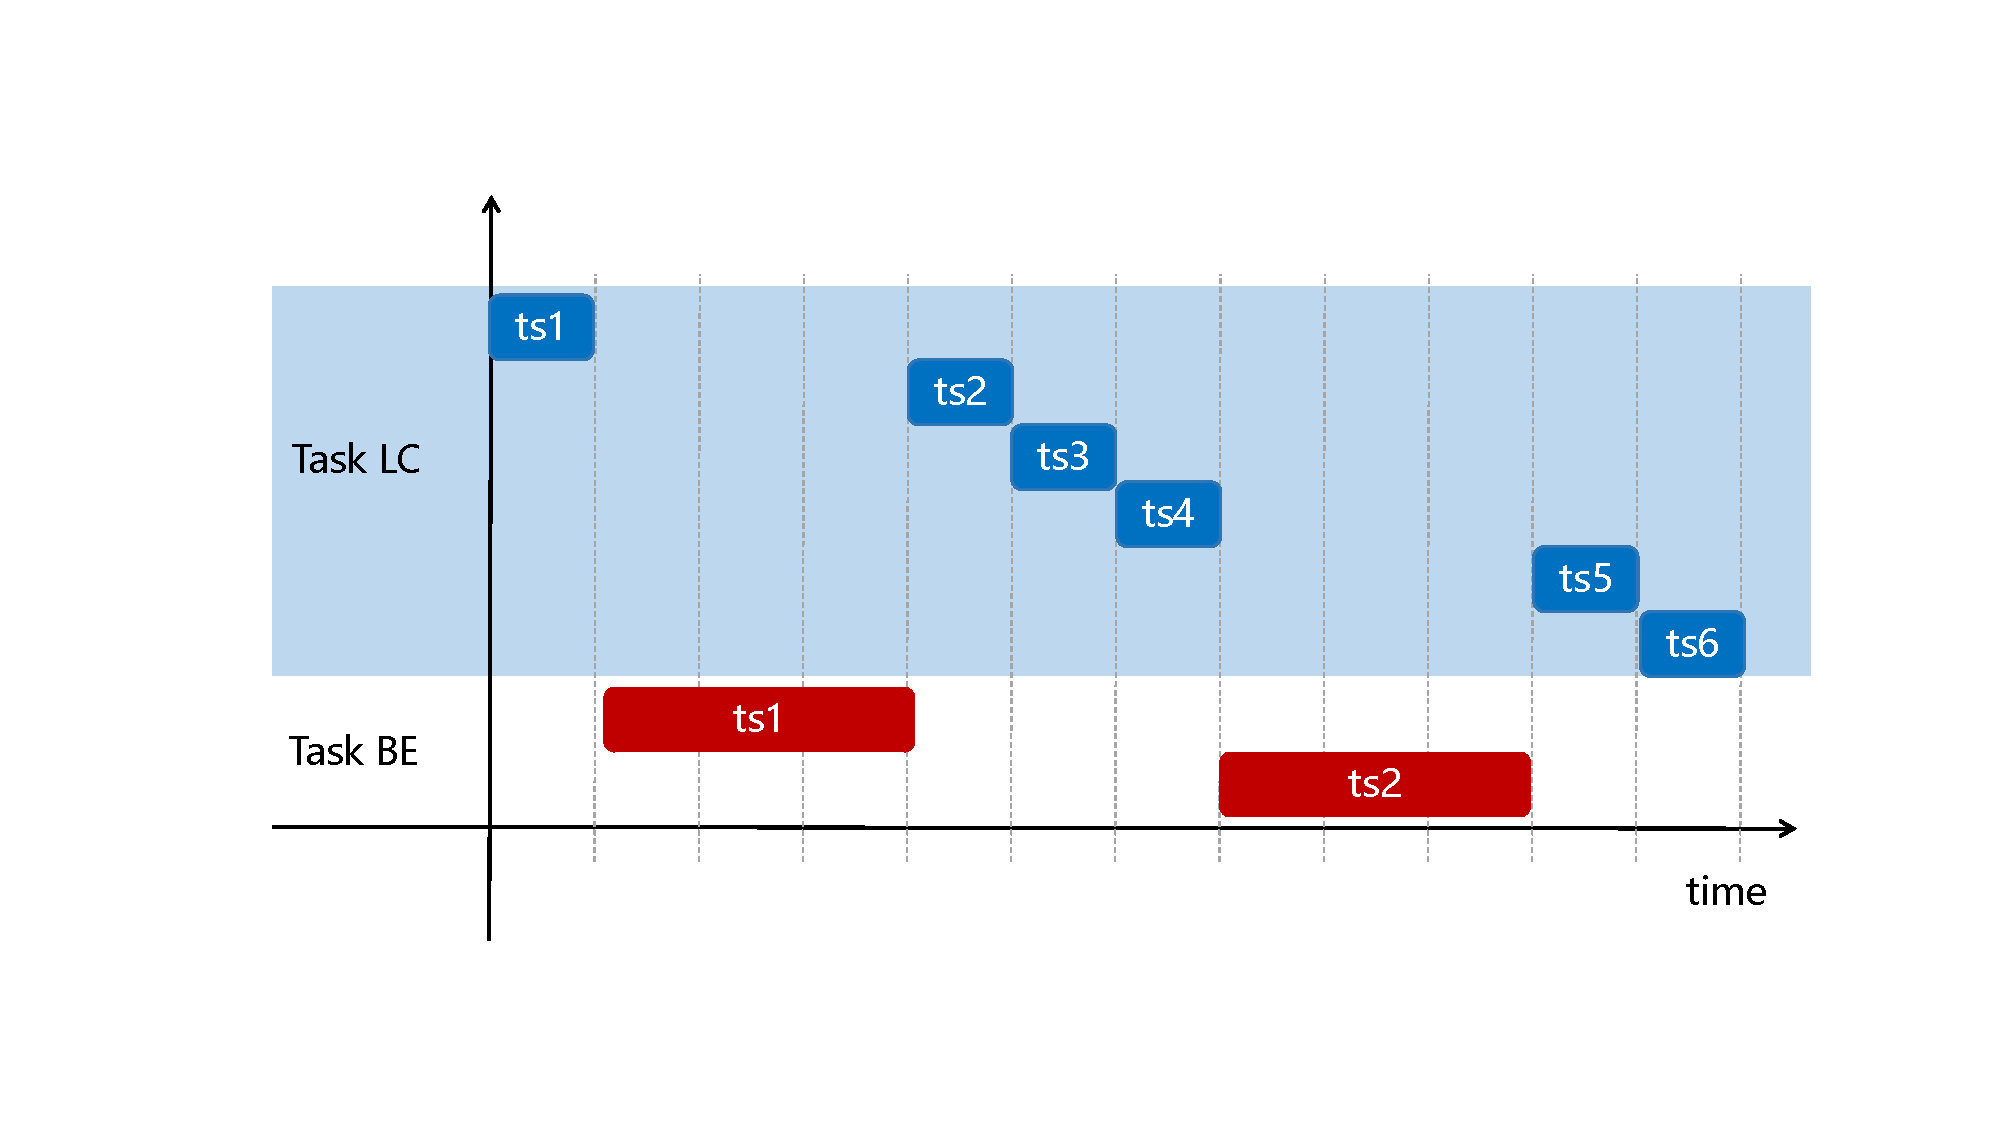
\includegraphics[width=0.65\textwidth]{eevdf_scheduling}
    \bicaption{\quad EEVDF可变时间片机制}{\quad EEVDF Variable Time Slice Mechanism}
    \label{fig:eevdf_scheduling}
\end{figure}

针对CPU拓扑,Linux 2.6中引入了调度域(Scheduler Domains)\citep{schedulerdomains},用来协助处理多核处理器上的调度。如表~\ref{tab:resourcesharing}所示,不同调度域充分反映了对于CPU拓扑上的资源共享信息。而调度子系统可基于调度域这层抽象来了解CPU间的差异性,进而针对性地进行调度。然而Linux任务调度机制在处理不同调度域时仍有不足:

\begin{itemize}
    \item 超线程调度域中兄弟核心存在如表~\ref{tab:resourcesharing}所示的共享资源,部署在兄弟核心上的应用存在竞争的可能。Elfen\citep{yang2016elfen}设计了一种新的内核调度机制,首先提供了一种全新的系统调用nanonap,允许进程快速地释放CPU资源但保留对CPU的所占有状态。同时,Elfen通过向BE应用插入探测代码,使得BE应用在运行过程中能够快速的探测兄弟核心上任务的运行并及时调用nanonap释放资源。通过以上设计,Elfen实现了LC应用与BE应用在部署到兄弟核心时的交替执行,从而避免因资源竞争导致的QoS劣化。 

    \begin{table}[!htbp]
        \bicaption{\quad 调度域与共享资源}{\quad scheduler domains and resource sharing}% caption
        \label{tab:resourcesharing}
        \footnotesize% fontsize
        \setlength{\tabcolsep}{4pt}% column separation
        \renewcommand{\arraystretch}{1.5}% row space 
        \centering
        \begin{tabular}{lc}
            \hline
            %\multicolumn{num_of_cols_to_merge}{alignment}{contents} \\
            %\cline{i-j}% partial hline from column i to column j
            调度域 & 共享资源\\
            \hline
            Core & 几乎隔离\\
            SMT & 执行单元、缓存、总线\\
            NUMA & 末级缓存、内存带宽、IO\\
            \hline
        \end{tabular}
    \end{table}

    \item 部分片上资源存在隐含的竞争破坏了调度域的隔离性。AVX(Advanced Vector Extensions)指令属于SIMD的一部分,旨在提高CPU的浮点运算性能,最早由Intel提出并于2011开始在实际产品中加入。AVX指令涉及到CPU中加速单元的使用,而使用加速单元意味着更高的能耗。为防止过热,现代CPU通常会在加速单元工作时降低运行频率。这就引发了两个Linux任务调度上的公平性问题\citep{gottschlag2020avx}。首先,由于CPU频率的恢复需要一定的时间,当同一Core调度域中的任务切换发生在恢复过程中时,就存在相互影响的可能。其次,兄弟核心共享了同一个物理核,物理核心的频率会使得所有兄弟核心受到影响。为解决这两个公平性问题,Gottschlag\citep{gottschlag2021fair}对现有调度机制进行了修改。首先,Gottschlag设计了一种监测手段,能够通过向量寄存器的使用情况来判断是否有AVX指令的执行。随后,Gottschlag在任务调度机制中增加了vruntime补偿逻辑,通过调整受影响的Core调度域与SMT调度域上的任务的vruntime来解决公平性问题。
\end{itemize}

另一种通过任务调度保障混部应用QoS的思路是微秒级调度\citep{ousterhout2019shenango,fried2020caladan,prekas2017zygos},其核心在于将调度延时降低到LC应用允许的延迟范围内,及时分配CPU资源来避免应用QoS劣化。Caladan\citep{fried2020caladan}实现了一种用户态的任务运行时,并通过DPDK(Data Plane Development Kit)、SPDK(Storage Performance Development Kit)解决硬件驱动问题。Caladan将操作系统的大部分功能实现到用户态,一方面去除了地址空间隔离,能够大大减少上下文切换的开销。另一方面打破Linux调度子系统的限制,能够更灵活地开发调度策略。Caladan使用集中式的调度模式,在负责调度的核心上基于高精度时钟实现微秒级调度延时。同时,Caladan能够从DPDK、SPDK中读取硬件资源的分配状况,这些额外信息能够有效辅助进行调度决策。

为特定工作负载量身定制调度策略能够显著改善如延时、吞吐量、能效等关键指标,然而在大型数据中心设计、实施和部署新的任务调度策略是一项艰巨的任务\citep{humphries2021ghost}。首先,调度子系统涉及Linux内核中的许多复杂机制,如复杂的同步原语及P-state(Processor State)控制等,独立开发的难度较大。其次,Linux内核开发不同于普通用户程序,可用程序库较少,且对代码编写有严格的限制与规范。部署新调度策略时,由于Linux无法在运行时重载调度子系统,因此通常需要重新启动。而服务器的重启意味着反复的任务迁移,这在生产环境是难以接受的。最后,Linux社区在调度子系统的迭代上相对保守,并期望实现普适的调度策略,一个高质量的调度器通常需要数十年的时间来不断完善\citep{agache2020firecracker},如EEVDF调度器从提出到正式并入主线内核就花费了29年。

为解决内核调度器在设计、实施和部署上的问题,加速内核调度机制迭代,Google提出了ghOSt\citep{humphries2021ghost}用户态调度器框架。ghOSt框架中包含三部分:内核调度类、用户态调度器及调度信息协议。其中,内核调度类在内核侧不断地更新任务状态,并按协议生成调度事件。用户态调度器通过特殊的系统调用消费事件并进行调度决策。而决策同样以事件的形式通过特殊系统调用提交到内核调度类,并进行真正地实施。ghOSt调度框架在一定程度上解决了内核调度的灵活性问题,但由于频繁系统调用所引发的上下文切换开销,难以实现较低的调度延时。eBPF技术提供了一种对Linux现有功能动态修改的思路,但仅在网络子系统中有较成熟的实践。Meta与内核社区的开发者共同创建了Sched Ext项目,提供了一种使用eBPF技术定制Linux调度机制的方式。相较于ghOSt,Sched Ext完全运行在内核中,能够实现更低的调度延时。同时,Sched Ext能够借助eBPF在其他子系统中的探测能力获取丰富的信息来辅助调度决策,实现更好地应用QoS保障。

\section{论文的研究内容}

本文主要研究单点混部场景QoS保障问题,综合以上相关理论研究能够发现:

\begin{enumerate}

    \item \textbf{数据中心传统应用划分形式单一,容易忽略应用在资源上的倾向性与敏感性}。这一方面容易引发混部应用在隐含资源上竞争,另一方面也不利于系统资源的充分利用。在观测指标上,相关研究表明单一指标在部分场景中有效,但同时也依赖多维度、广泛的数据采集来对应用进行充分性能分析。最后,AI技术在集群调度上能够很好的发挥作用,但对于节点侧尤其是内核调度上,AI技术存在实施与部署上困难的问题。
    
    \item \textbf{任务调度机制是解决单点混部场景QoS保障问题的核心}。数据中心LC应用大部分为服务型应用,其资源使用倾向与敏感度随负载变化而变化。负载的动态性要求调度机制能够迅速的做出反应。基于资源隔离的调度程序一般在用户态实现,依赖系统调用来获取资源分配信息和进行资源隔离。同时,资源隔离机制存在一定的生效延迟。这都限制了调度程序的调度频率,不利于应用的QoS保障。不同于资源隔离,任务调度则通过CPU资源分配来间接地控制应用的资源使用。尽管调控粒度较粗,但由于在调度速度上的优势,任务调度能够更好地在单点上保障混部应用的QoS。
    
    \item \textbf{应用动态特性要求更灵活的任务调度机制,且单一的任务调度机制无法在各个混部场景有效}。Linux内核追求普适的调度机制,并存在大量的启发式逻辑,难以针对特定混部场景进行调整与定制。其次,Linux调度机制在编译时确定且无法在运行时修改,在软硬件环境发生变化时不能快速调整。微秒级任务调度机制虽然QoS保障效果优秀,但由于绕过内核的设计与高度的定制,存在兼容性问题,无法在生产环境中大规模使用。最后,服务器资源丰富,能够同时运行大量应用,这些应用构成多样的混部场景。而相关研究通常针对特定的混部场景,无法保证在各个混部场景下有效。

\end{enumerate}

综合上述对混部场景QoS保障研究的分析,本文总结了如下挑战并开展相应工作:

\begin{enumerate}

    \item \textbf{针对数据中心的软件环境复杂性挑战,展开典型应用监测与画像分析研究}。首先,结合对数据中心软件栈分析以及与云厂商的合作经验,选择了一批典型应用作为画像目标,并采用虚拟机作为应用的运行环境。随后,设计实现了一套可观测性系统,围绕虚拟机在Host、Hypervisor与App等多重维度,采集丰富的指标信息。最后,在可观测性系统的基础之上,展开针对典型应用的资源倾向与敏感度实验并给出画像结论。

    \item \textbf{针对当前任务调度机制在不同混部场景下的不足,展开混部场景导向的定制任务调度机制研究}。首先,从内核任务调度的相关配置上针对不同应用的需求,设计了响应度优先与吞吐量优先两种基础内核配置。随后,在Ext调度类的基础上设计了塔台(Control Tower)任务调度框架,并在此基础上,结合eBPF技术的监测能力进一步实现CPU资源感知与网络资源感知的任务调度策略。

    \item \textbf{针对单一调度机制与多样混部场景的挑战,设计实现受控空域(Contorl Zone),一种面向混部场景的调度动态可定制沙箱}。Control Zone基于KVM虚拟机实现,如图~\ref{fig:arch_dif}所示,相较于Firecracker\citep{agache2020firecracker},Control Zone允许将Control Tower调度策略与混部应用协同部署。一方面,能够针对不同混部场景自由地选择合适的Control Tower调度策略。另一方面,能够随混部应用的变化在运行时对Control Tower调度器动态修改。同时,还支持通过软硬件手段来隔离不同Control Zone的资源。

\end{enumerate}

\begin{figure}[!htbp]
    \centering
    \begin{subfigure}[b]{0.4\textwidth}
        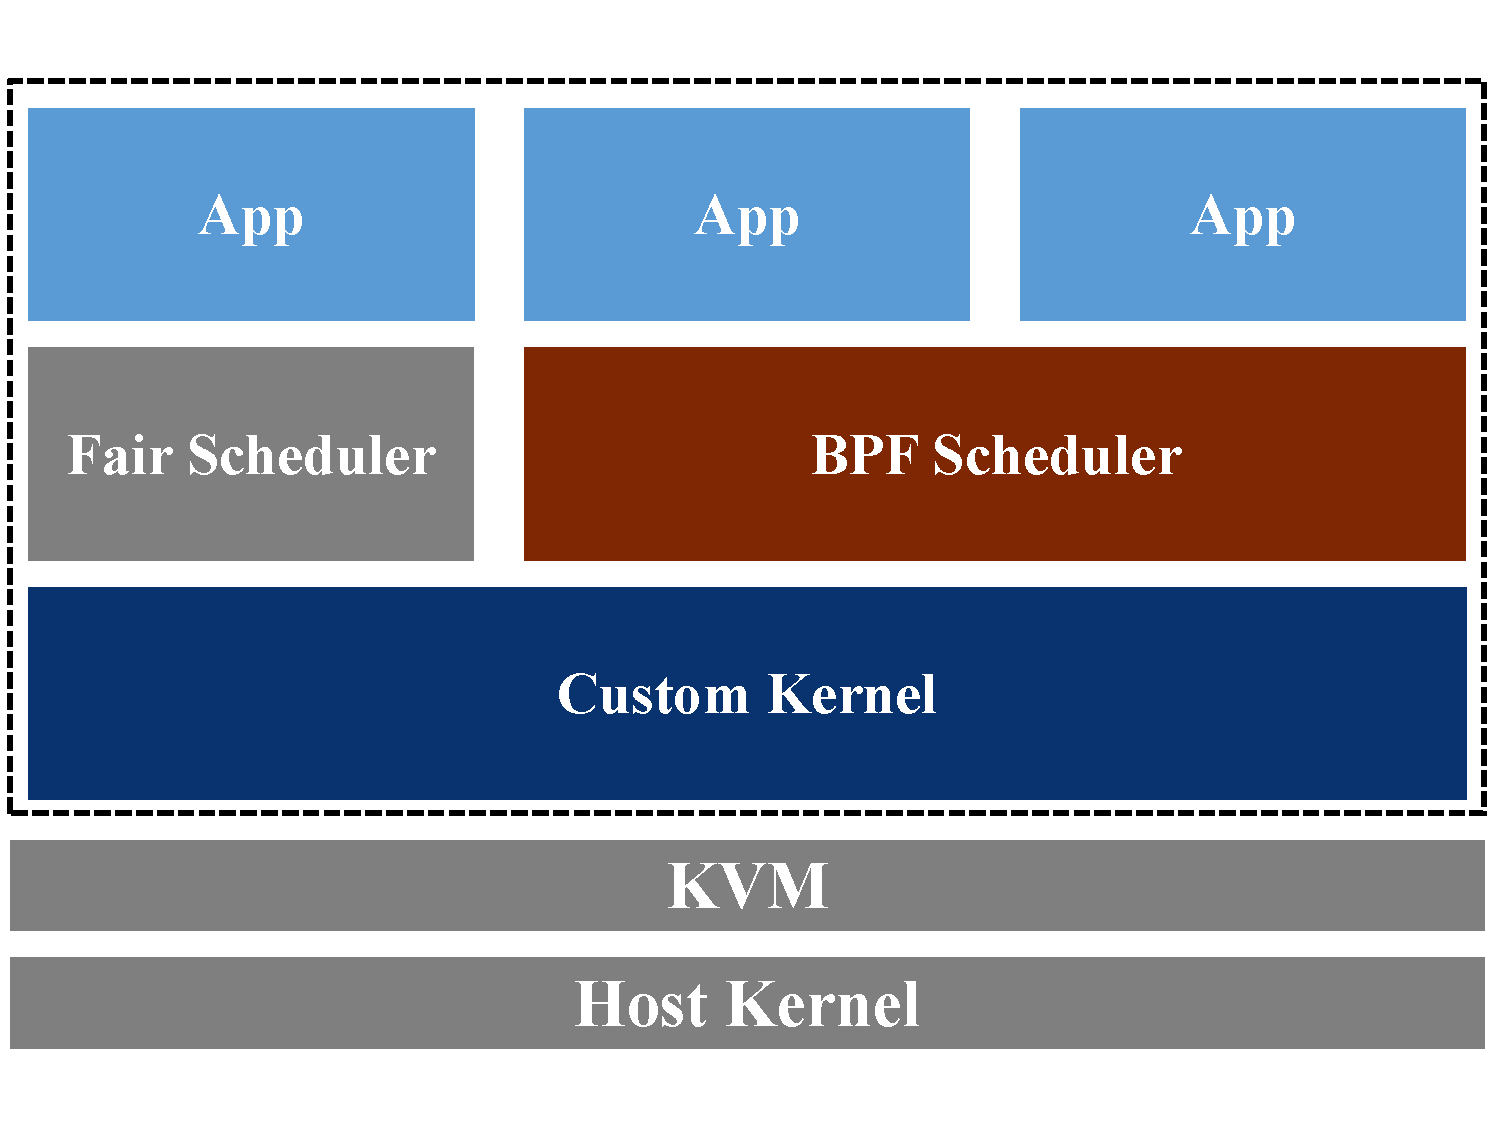
\includegraphics[width=\textwidth]{arch_dif_cz}
        \caption{Control Zone}
        \label{fig:arch_dif_cz}
    \end{subfigure}
    \hspace{0.5cm}
    \begin{subfigure}[b]{0.4\textwidth}
        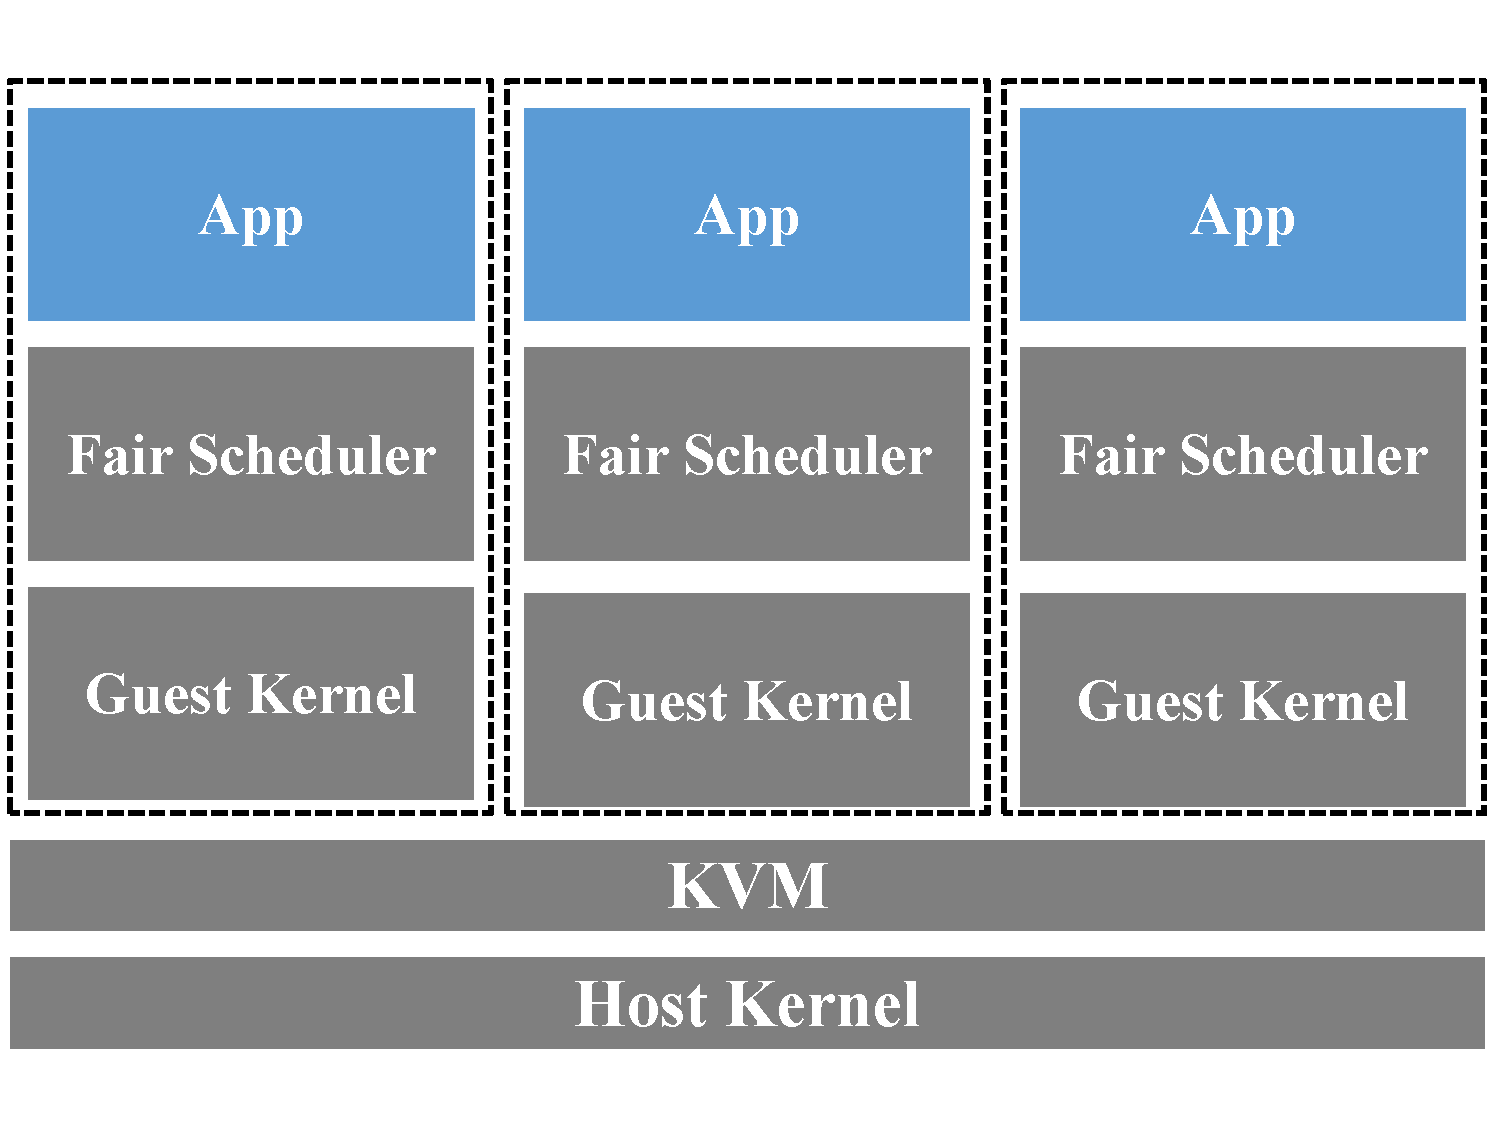
\includegraphics[width=\textwidth]{arch_dif_fc}
        \caption{Firecracker}
        \label{fig:arch_dif_fc}
    \end{subfigure}
\bicaption{\quad 沙箱结构差异}{\quad Sandbox Structure Differences}
\label{fig:arch_dif}
\end{figure}

\section{论文结构安排}

本文的主要内容分为六章,总体结构如图~\ref{fig:paper_organization}所示:

\begin{figure}[!htbp]
    \centering
    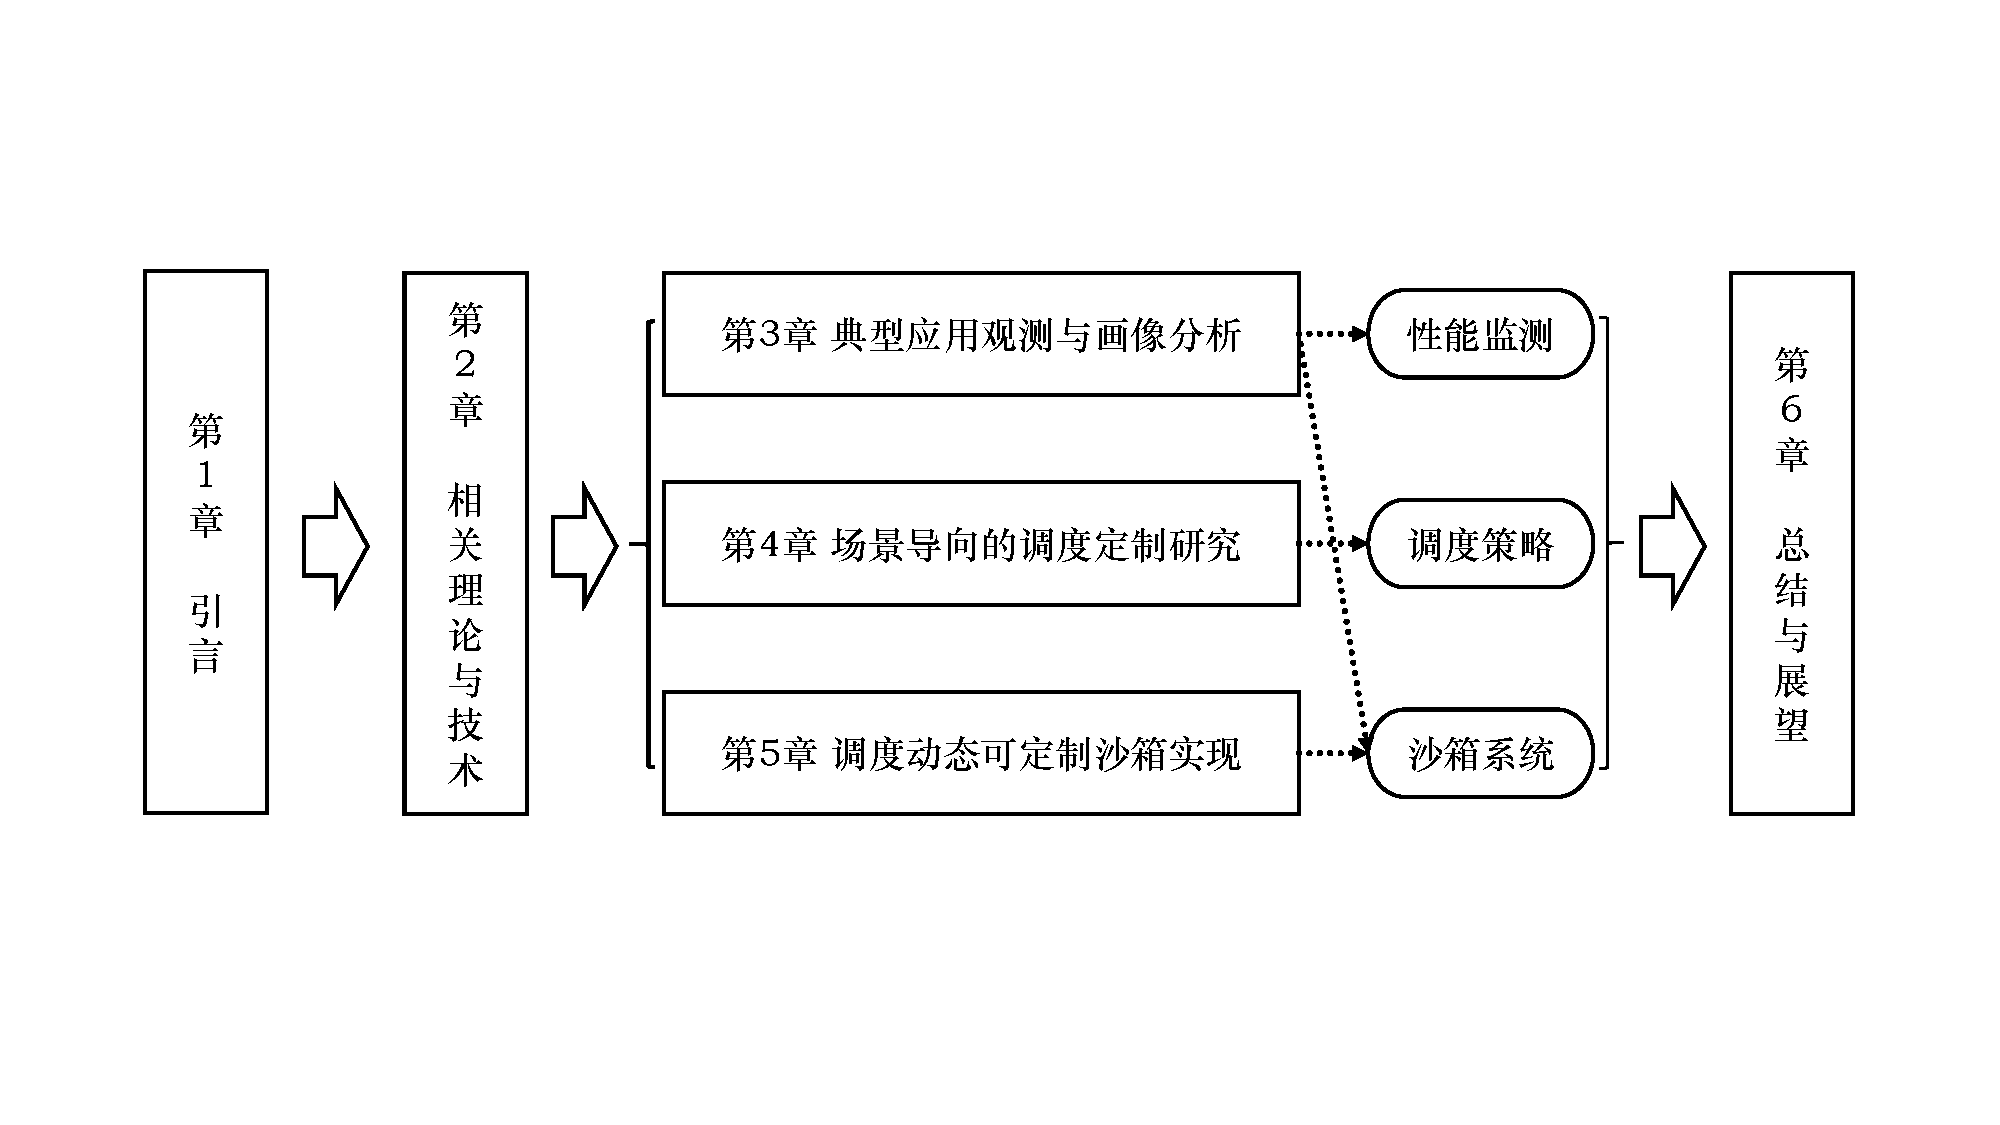
\includegraphics[width=0.8\textwidth]{paper_organization}
    \bicaption{\quad 本文组织架构}{\quad Paper Organization}
    \label{fig:paper_organization}
\end{figure}

第1章,相关背景说明。首先,阐述了本文的主要背景,以及面向混部场景的QoS保障问题。随后,从可观测性与劣化监测、围绕资源隔离的混部场景QoS保障、围绕任务调度的混部场景QoS保障三个方面分析了国内外研究现状。最后,阐述了本文研究所面临的挑战以及要展开的各项工作。

第2章,本文中所使用到的技术说明。首先,分析了经典的Linux调度子系统的构成以及任务调度的决策过程。其次,介绍了本文中使用到的eBPF技术,阐述其核心特点,以及相较于内核模块等传统内核功能扩展技术的差异。随后,介绍了Sched Ext项目,一种插件化内核调度器补丁集,说明了其实现的原理。最后,介绍了沙箱技术以及相关的实现。

第3章,典型应用观测与画像分析。首先,介绍了云场景典型应用以及应用运行环境的选择。其次,阐述了针对KVM虚拟机的多维度指标采集可观测性系统的设计与实现。最后,分别对基准性能实验与干扰敏感度实验进行实验设计的阐述与最后的画像结果分析。

第4章,混部场景导向的任务调度机制定制,包含内核配置定制、Control Tower任务调度框架两个方面。在内核调度配置上,设计了响应度优先与吞吐量优先两种内核配置。在Control Tower任务调度框架上,首先阐述了设计目标和实现原理,以及CPU资源感知与网络资源感知两种调度策略的实现。最后,设计实验验证场景导向的调度机制在应用QoS保障上的效果。

第5章,Control Zone的设计与实现。在第3、4章的基础上,设计实现了一种调度动态可定制沙箱。一方面能够通过内核调度定制与Control Tower任务调度框架,针对混部场景选择合适的任务调度机制。另一方面基于虚拟化,实现不同调度机制在同一物理机上共存。最后,设计实验说明沙箱的开销以及在混部场景下保障应用QoS的效果。

第6章,总结与展望。首先对于本文针对混部场景QoS保障问题的三个工作进行总结,分析了本文工作的效果与不足之处。随后,对利用eBPF观测能力与Ext调度类灵活性在更多混部场景定制Control Tower调度策略进行了展望。